
许多脚本语言都具有一个将两个序列压缩在一起的函数,zip操作就可以接受两个输入序列,并为两个输入中的每个位置返回一对值:

考虑两个序列的情况——可以是容器、迭代器或初始化列表:

\hspace*{\fill} \\ %插入空行
\begin{center}
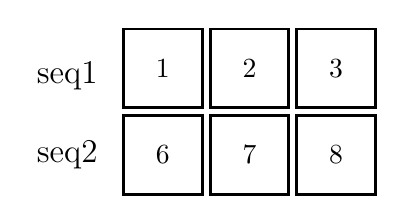
\begin{tikzpicture}
\foreach \x in {1,...,3} {
	\draw[line width=1pt] (1.1*\x,1) rectangle (1.1*\x+1,0) node[pos=.5] {\x};
}

\foreach \x [evaluate=\x as \index using int(\x+5)] in {1,...,3} {
	\draw[line width=1pt] (1.1*\x,-0.1) rectangle (1.1*\x+1,-1.1) node[pos=.5] {\index};
}

\node[text width=3cm, font=\large] at (1.5, 0.4) {seq1};
\node[text width=3cm, font=\large] at (1.5,-0.6) {seq2};
\end{tikzpicture}

图4.6 需要压缩的容器
\end{center}

我们想把它们压缩在一起,用前两个序列中的元素对组成一个新序列:

\hspace*{\fill} \\ %插入空行
\begin{center}
\begin{tikzpicture}
\node[text width=3cm, font=\large] at (1.2, 0.4) {seq1};
\node[text width=3cm, font=\large] at (1.2,-0.6) {seq2};
\node[text width=3cm, font=\large] at (0.9,-2.5) {zipped};

\draw[line width=1pt] (1,1) rectangle (2,0) node[pos=.5] {1};
\draw[line width=1pt] (3.5,1) rectangle (4.5,0) node[pos=.5] {2};
\draw[line width=1pt] (6,1) rectangle (7,0) node[pos=.5] {3};

\draw[line width=1pt] (2.1,-0.2) rectangle (3.1,-1.2) node[pos=.5] {6};
\draw[line width=1pt] (4.6,-0.2) rectangle (5.6,-1.2) node[pos=.5] {7};
\draw[line width=1pt] (7.1,-0.2) rectangle (8.1,-1.2) node[pos=.5] {8};

\draw[line width=1pt] (1,-3.0) rectangle (2,-2.0) node[pos=.5] {1};
\draw[line width=1pt] (2.1,-3.0) rectangle (3.1,-2.0) node[pos=.5] {6};

\draw[line width=1pt] (3.5,-3.0) rectangle (4.5,-2.0) node[pos=.5] {2};
\draw[line width=1pt] (4.6,-3.0) rectangle (5.6,-2.0) node[pos=.5] {7};

\draw[line width=1pt] (6,-3.0) rectangle (7,-2.0) node[pos=.5] {3};
\draw[line width=1pt] (7.1,-3.0) rectangle (8.1,-2.0) node[pos=.5] {8};


\draw[decorate,decoration={calligraphic brace,amplitude=2mm, mirror},ultra thick] (1.5,-3.2) -- (2.6,-3.2);
\draw[decorate,decoration={calligraphic brace,amplitude=2mm, mirror},ultra thick] (4,-3.2) -- (5.1,-3.2);
\draw[decorate,decoration={calligraphic brace,amplitude=2mm, mirror},ultra thick] (6.5,-3.2) -- (7.6,-3.2);

\draw[line width=2pt][-latex] (1.5,-0.1) -- (1.5,-1.9);
\draw[line width=2pt][-latex] (2.6,-1.3) -- (2.6,-1.9);

\draw[line width=2pt][-latex] (4,-0.1) -- (4,-1.9);
\draw[line width=2pt][-latex] (5.1,-1.3) -- (5.1,-1.9);

\draw[line width=2pt][-latex] (6.5,-0.1) -- (6.5,-1.9);
\draw[line width=2pt][-latex] (7.6,-1.3) -- (7.6,-1.9);

\node[text width=3cm, font=\large] at (3.2,-3.7) {pair};
\node[text width=3cm, font=\large] at (5.7,-3.7) {pair};
\node[text width=3cm, font=\large] at (8.2,-3.7) {pair};
\end{tikzpicture}

图4.7  Zip操作
\end{center}

示例中,将使用迭代器适配器来完成这项任务。

\subsubsection{How to do it…}

这个示例中,将构建一个zip迭代器适配器,接受两个相同类型的容器,并将值压缩到std::pair对象中:

\begin{itemize}
\item 
main()函数中,可以用两个vector来调用适配器:

\begin{lstlisting}[style=styleCXX]
int main()
{
	vector<std::string> vec_a {"Bob", "John", "Joni"};
	vector<std::string> vec_b {"Dylan", "Williams",
		"Mitchell"};
	cout << "zipped: ";
	for(auto [a, b] : zip_iterator(vec_a, vec_b)) {
		cout << format("[{}, {}] ", a, b);
	}
	cout << '\n';
}
\end{lstlisting}

可以使用zip\_iterator来代替单独的vector迭代器。

期望输出如下所示:

\begin{tcblisting}{commandshell={}}
zipped: [Bob, Dylan] [John, Williams] [Joni, Mitchell]
\end{tcblisting}

\item 
迭代器适配器在一个名为zip\_iterator的类中。为了方便起见,我们将从一些类型别名开始:

\begin{lstlisting}[style=styleCXX]
template<typename T>
class zip_iterator {
	using val_t = typename T::value_type;
	using ret_t = std::pair<val_t, val_t>;
	using it_t = typename T::iterator;
\end{lstlisting}

\item 
迭代器中不存储数据,只存储目标容器的begin()和end()迭代器的副本:

\begin{lstlisting}[style=styleCXX]
it_t ita_{};
it_t itb_{};
// for begin() and end() objects
it_t ita_begin_{};
it_t itb_begin_{};
it_t ita_end_{};
it_t itb_end_{};
\end{lstlisting}

ita\_和itb\_是目标容器的迭代器,其他四个迭代器用于为zip\_iterator适配器生成begin()和end()迭代器。

\item 
还有一个私有的构造函数:

\begin{lstlisting}[style=styleCXX]
// private constructor for begin() and end() objects
zip_iterator(it_t ita, it_t itb) : ita_{ita}, itb_{itb}
{}
\end{lstlisting}

稍后将用于构造专门用于begin()和end()迭代器的适配器对象。

\item 
public部分,从迭代器特性类型定义开始:

\begin{lstlisting}[style=styleCXX]
public:
using iterator_concept =
	std::forward_iterator_tag;
using iterator_category =
	std::forward_iterator_tag;
using value_type = std::pair<val_t, val_t>;
using difference_type = long int;
using pointer = const val_t*;
using reference = const val_t&;
\end{lstlisting}

\item 
构造函数设置所有私有迭代器变量:

\begin{lstlisting}[style=styleCXX]
zip_iterator(T& a, T& b) :
	ita_{a.begin()},
	itb_{b.begin()},
	ita_begin_{ita_},
	itb_begin_{itb_},
	ita_end_{a.end()},
	itb_end_{b.end()}
{}
\end{lstlisting}

\item 
定义了用于前向迭代器的最小操作符重载:

\begin{lstlisting}[style=styleCXX]
zip_iterator& operator++() {
	++ita_;
	++itb_;
	return *this;
}
bool operator==(const zip_iterator& o) const {
	return ita_ == o.ita_ || itb_ == o.itb_;
}
bool operator!=(const zip_iterator& o) const {
	return !operator==(o);
}
ret_t operator*() const {
	return { *ita_, *itb_ };
}
\end{lstlisting}

\item 
最后,begin()和end()函数返回各自的迭代器:

\begin{lstlisting}[style=styleCXX]
zip_iterator begin() const
	{ return zip_iterator(ita_begin_, itb_begin_); }
zip_iterator end() const
	{ return zip_iterator(ita_end_, itb_end_); }
\end{lstlisting}

存储的迭代器和私有构造函数使这些函数变得简单。

\item 
现在展开main()函数进行测试:

\begin{lstlisting}[style=styleCXX]
int main()
{
	vector<std::string> vec_a {"Bob", "John", "Joni"};
	vector<std::string> vec_b {"Dylan", "Williams",
		"Mitchell"};
	
	cout << "vec_a: ";
	for(auto e : vec_a) cout << format("{} ", e);
	cout << '\n';
	
	cout << "vec_b: ";
	for(auto e : vec_b) cout << format("{} ", e);
	cout << '\n';
	
	cout << "zipped: ";
	for(auto [a, b] : zip_iterator(vec_a, vec_b)) {
		cout << format("[{}, {}] ", a, b);
	}
	cout << '\n';
}
\end{lstlisting}


\item 
这给了我们期望的输出:

\begin{tcblisting}{commandshell={}}
vec_a: Bob John Joni
vec_b: Dylan Williams Mitchell
zipped: [Bob, Dylan] [John, Williams] [Joni, Mitchell]
\end{tcblisting}

\end{itemize}

\subsubsection{How it works…}

压缩迭代器适配器是迭代器抽象可以多么灵活的一个例子,可以获取两个容器的迭代器,并在一个聚合迭代器中使用。

zip\_iterator类的主构造函数接受两个容器对象。为了便于讨论,我们将这些对象称为目标对象。

\begin{lstlisting}[style=styleCXX]
zip_iterator(T& a, T& b) :
	ita_{a.begin()},
	itb_{b.begin()},
	ita_begin_{ita_},
	itb_begin_{itb_},
	ita_end_{a.end()},
	itb_end_{b.end()}
{}
\end{lstlisting}

构造函数从目标begin()迭代器初始化ita\_和itb\_变量,这些将用于导航目标对象。目标begin()和end()迭代器也会保存以供后续使用。

这些变量在private部分定义:

\begin{lstlisting}[style=styleCXX]
it_t ita_{};
it_t itb_{};
// for begin() and end() objects
it_t ita_begin_{};
it_t itb_begin_{};
it_t ita_end_{};
it_t itb_end_{};
\end{lstlisting}

it\_t类型定义为目标迭代器类的类型:

\begin{lstlisting}[style=styleCXX]
using val_t = typename T::value_type;
using ret_t = std::pair<val_t, val_t>;
using it_t = typename T::iterator;
\end{lstlisting}

其他别名类型是val\_t,表示目标值的类型,ret\_t表示返回值对,整个类中使用这些类型定义是为了方便使用。

begin()和end()函数使用只初始化ita\_和itb\_值的私有构造函数:

\begin{lstlisting}[style=styleCXX]
zip_iterator begin() const
	{ return zip_iterator(ita_begin_, itb_begin_); }
zip_iterator end() const
	{ return zip_iterator(ita_end_, itb_end_); }
\end{lstlisting}

私有构造函数:

\begin{lstlisting}[style=styleCXX]
// private constructor for begin() and end() objects
zip_iterator(it_t ita, it_t itb) : ita_{ita}, itb_{itb} {}
\end{lstlisting}

这是一个使用it\_t迭代器作为参数的构造函数,只初始化ita\_和itb\_,以便在比较操作符重载中使用。

类的其余部分就像普通的迭代器一样,但操作的是目标类的迭代器:

\begin{lstlisting}[style=styleCXX]
zip_iterator& operator++() {
	++ita_;
	++itb_;
	return *this;
}
bool operator==(const zip_iterator& o) const {
	return ita_ == o.ita_ || itb_ == o.itb_;
}
bool operator!=(const zip_iterator& o) const {
	return !operator==(o);
}
\end{lstlisting}

解引用操作符返回一个std::pair对象(ret\_t是std::pair<val\_t, val\_t>的别名)。这是从迭代器接口中检索出的值。

\begin{lstlisting}[style=styleCXX]
ret_t operator*() const {
	return { *ita_, *itb_ };
}
\end{lstlisting}

\subsubsection{There's more…}

zip\_iterator适配器可以用来将对象压缩到map中:

\begin{lstlisting}[style=styleCXX]
map<string, string> name_map{};

for(auto [a, b] : zip_iterator(vec_a, vec_b)) {
	name_map.try_emplace(a, b);
}

cout << "name_map: ";
for(auto [a, b] : name_map) {
	cout << format("[{}, {}] ", a, b);
}
cout << '\n';
\end{lstlisting}

若将这段代码添加到main(),则会得到这样的输出:

\begin{tcblisting}{commandshell={}}
name_map: [Bob, Dylan] [John, Williams] [Joni, Mitchell]
\end{tcblisting}












